\documentclass[a4paper, 12pt, english, brazilian]{article}
\usepackage{graphicx}

\usepackage{imegoodies}
\usepackage{imelooks}
\usepackage{amsmath}
\usepackage{amsfonts}
\usepackage{forest}
\usepackage{tikz}
\usepackage{float}
\raggedbottom % Verificar isso

\title{Relatório IC - Estruturas de Dados Probabilísticas e Compactas}
\author{Bruno Rangel Pereira Tadim}
\date{\today}

\begin{document}

\maketitle

\section{Introdução}
Esse projeto de pesquisa visa estudar os fundamentos de estruturas probabilísticas e compactas, 
incluindo estruturas clássicas da área, suas respectivas vantagens e desvantagens, além de realizar implementações
para experimentação empírica.

\section{Entropia}
A entropia de uma estrutura de dados é o limite mínimo de bits necessários para representar 
todos os possíveis estados que essa estrutura pode assumir.

A Teoria da Informação de Shannon nos diz que, se temos uma estrutura de dados com conjunto 
de estados $U$, onde cada estado $u \in U$ possui probabilidade de ocorrência $\Pr(u)$, dada por uma função $\Pr : U \to [0, 1]$
a entropia $\mathcal{H}(\Pr)$ é definida como:
\[
    \mathcal{H}(\Pr) = -\sum_{u \in U}{\Pr(u)\log\Pr(u)} = \sum_{u \in U}{\Pr(u)\log\frac{1}{\Pr(u)}}
\]
Denominamos esse valor como entropia de Shannon.

Se a probabilidade de ocorrência for igual $\forall u \in U$, ou seja, $\Pr(u) = \frac{1}{|U|}$, 
então o cálculo de $\mathcal{H}(\Pr)$ será

\begin{align*}
    \mathcal{H}(\Pr) &= -\sum_{u \in U}{\frac{1}{|U|}\log\frac{1}{|U|}} 
    = \frac{1}{|U|} \left(-\sum_{u \in U}{\log\frac{1}{|U|}}\right)\\
    &= \frac{1}{|U|} \left( -|U| \log\frac{1}{|U|} \right) = -\log\frac{1}{|U|} = \log|U|
\end{align*}

Chamamos o caso acima de \textit{worst-entropy} e o denotamos $\mathcal{H}_{wc}$, pois o maior valor de $\mathcal{H}$ é
obtido quando a distribuição de probabilidade é uniforme.  Nesse caso, dizemos que o 
conjunto $U$ é incompressível.

Para representarmos os elementos do conjunto $U$, atribuímos um código binário a cada um deles.
Se todos os códigos tiverem o mesmo tamanho $l$, então o número de bits necessários será 
$\log|U| = \mathcal{H}_{wc}(U)$. Caso $l <\mathcal{H}_{wc}$, teríamos apenas $2^{l} < 2^{\mathcal{H}_{wc}}
= 2^{\log|U|} = |U|$ códigos distintos, o que é insuficiente para representar todos os $|U|$ elementos.

No entanto, caso tenhamos informações sobre a distribuição de probabilidade $\Pr$ associada a $U$, e ela não
for uniforme, podemos reduzir essa quantidade. Considere um conjunto $U = \{u_1, u_2, u_3, u_4\}$,
com probabilidades $\{0.6, 0.2, 0.15, 0.05\}$, respectivamente. A entropia nesse caso é $\mathcal{H}(U) = 
0.6 \cdot \log\frac{1}{0.6} + 0.2 \cdot \log\frac{1}{0.2} 
+ 0.15 \cdot \log\frac{1}{0.15} + 0.05 \cdot \log\frac{1}{0.05} \approx 1.5332 < \log4 = 2 = \mathcal{H}_{wc}(U)$.

Podemos atribuir o código \texttt{0} para $u_1$, \texttt{10} para $u_2$, \texttt{110} para $u_3$ e \texttt{111}
para $u_4$. Dessa forma, o tamanho médio dos códigos será $0.6 \cdot 1 + 0.2 \cdot 2 + 0.15 \cdot 3 
+ 0.05 \cdot 3 = 1.6$ bits, o que é próximo da entropia mínima e menor que o pior caso.

É importante que a codificação seja livre de prefixos, ou seja, nenhum código pode ser prefixo de outro, caso
contrário, será impossível realizar a decodificação sem ambiguidades. Os códigos escolhidos acima foram gerados
utilizando a \textbf{codificação de Huffman}.

\subsection{Codificação de Huffman}
A codificação de Huffman é um algoritmo que, dada uma distribuição de probabilidade $\Pr : \Sigma \to [0.0, 1.0]$, 
retorna um código de prefixo que minimiza o tamanho médio dos códigos.

O algoritmo opera de forma gulosa e transforma um conjunto de $|\Sigma|$ nós em uma árvore binária. Inicialmente, temos
um nó isolado para cada símbolo $s \in \Sigma$, contendo como valor a sua respectiva probabilidade $\Pr(s)$. A cada passo, as duas raízes
de menores probabilidades são mescladas, se tornando ambas filhas de uma nova raíz, que conterá como valor a soma
dessas probabilidades.

\begin{figure}[H]
    \centering
    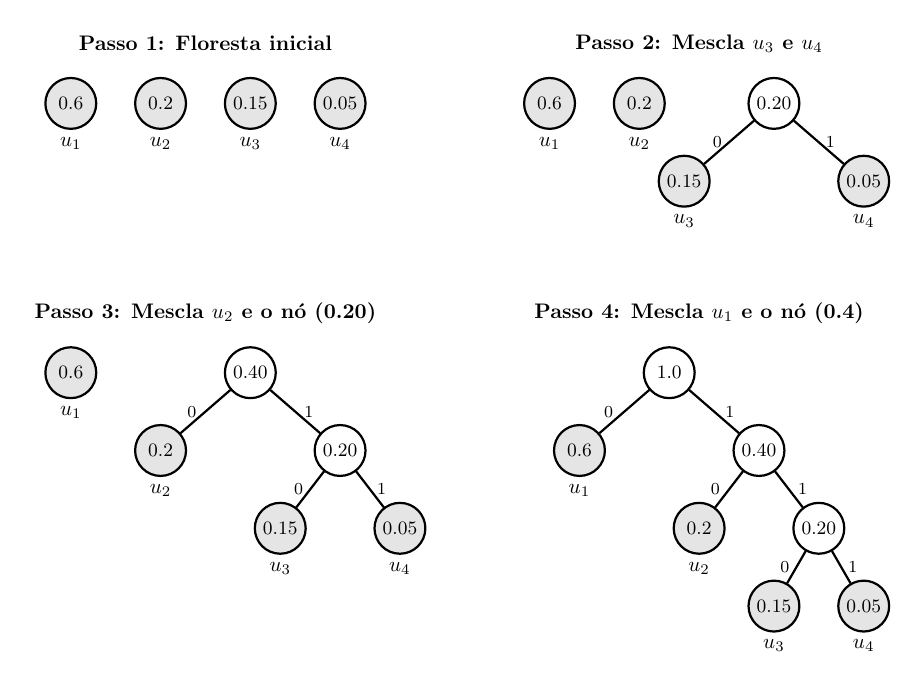
\begin{tikzpicture}[
        scale=0.76, transform shape,
        tnode/.style={circle, draw, thick, minimum size=8.5mm, inner sep=0pt, font=\small},
        leaf/.style={tnode, fill=gray!20},
        edge from parent/.style={draw, thick},
        lbl/.style={draw=none, fill=none, font=\footnotesize, inner sep=2pt},
        level 1/.style={sibling distance=3cm, level distance=1.3cm},
        level 2/.style={sibling distance=2cm, level distance=1.3cm},
        level 3/.style={sibling distance=1.5cm, level distance=1.3cm}
    ]

    % Passo 1
    \begin{scope}[xshift=0cm, yshift=0cm]
        \node[draw=none, font=\bfseries] at (2.25, 1) {Passo 1: Floresta inicial};
        \node[leaf, label=below:{$u_1$}] at (0,0) {0.6};
        \node[leaf, label=below:{$u_2$}] at (1.5,0) {0.2};
        \node[leaf, label=below:{$u_3$}] at (3,0) {0.15};
        \node[leaf, label=below:{$u_4$}] at (4.5,0) {0.05};
    \end{scope}

    % Passo 2
    \begin{scope}[xshift=8cm, yshift=0cm]
        \node[draw=none, font=\bfseries] at (2.5, 1) {Passo 2: Mescla $u_3$ e $u_4$};
        \node[leaf, label=below:{$u_1$}] at (0,0) {0.6};
        \node[leaf, label=below:{$u_2$}] at (1.5,0) {0.2};
        \node[tnode] at (3.75,0) {0.20}
            child {node[leaf, label=below:{$u_3$}] {0.15} edge from parent node[left, lbl, xshift=-1pt] {0}}
            child {node[leaf, label=below:{$u_4$}] {0.05} edge from parent node[right, lbl, xshift=1pt] {1}};
    \end{scope}

    % Passo 3
    \begin{scope}[xshift=0cm, yshift=-4.5cm]
        \node[draw=none, font=\bfseries] at (2.25, 1) {Passo 3: Mescla $u_2$ e o nó (0.20)};
        \node[leaf, label=below:{$u_1$}] at (0,0) {0.6};
        \node[tnode] at (3,0) {0.40}
            child {node[leaf, label=below:{$u_2$}] {0.2} edge from parent node[left, lbl, xshift=-2pt] {0}}
            child {node[tnode] {0.20}
                child {node[leaf, label=below:{$u_3$}] {0.15} edge from parent node[left, lbl, xshift=-1pt] {0}}
                child {node[leaf, label=below:{$u_4$}] {0.05} edge from parent node[right, lbl, xshift=1pt] {1}}
            edge from parent node[right, lbl, xshift=2pt] {1}};
    \end{scope}

    % Passo 4
    \begin{scope}[xshift=8cm, yshift=-4.5cm]
        \node[draw=none, font=\bfseries] at (2.5, 1) {Passo 4: Mescla $u_1$ e o nó (0.4)};
        \node[tnode] at (2,0) {1.0}
            child {node[leaf, label=below:{$u_1$}] {0.6} edge from parent node[left, lbl, xshift=-3pt] {0}}
            child {node[tnode] {0.40}
                child {node[leaf, label=below:{$u_2$}] {0.2} edge from parent node[left, lbl, xshift=-2pt] {0}}
                child {node[tnode] {0.20}
                    child {node[leaf, label=below:{$u_3$}] {0.15} edge from parent node[left, lbl, xshift=-1pt] {0}}
                    child {node[leaf, label=below:{$u_4$}] {0.05} edge from parent node[right, lbl, xshift=1pt] {1}}
                edge from parent node[right, lbl, xshift=2pt] {1}}
            edge from parent node[right, lbl, xshift=3pt] {1}};
    \end{scope}

    \end{tikzpicture}
    \caption{Execução passo a passo do algoritmo de Huffman para o conjunto $U$.}
    \label{fig:huffman_steps}
\end{figure}

A árvore final gerada pelo algoritmo é denominada \textit{árvore de Huffman}. Partindo da raíz da árvore, interpretamos 
ir para esquerda como \texttt{0} e ir para direita como \texttt{1}. Dessa forma, o caminho da raíz da árvore até uma folha
$s \in \Sigma$ representa o código referente a $s$, $\mathcal{C}(s)$. A árvore de Huffman minimiza o tamanho médio dos
códigos, dado por $\sum_{s \in \Sigma}{\Pr(s)l(s)}$.

Ao implementarmos o algoritmo, podemos inserir os elementos em uma lista de prioridade (\textit{Min-Heap}), ordenada
pelas probabilidades. A cada iteração, extraímos os dois nós de peso mínimo, criamos um novo nó interno com a soma 
de suas probabilidades e o reinserimos na fila. Como cada operação de extração e inserção na fila de prioridade 
tem custo $\mathcal{O}(\log|\Sigma|)$ e o processo se repete até restar apenas um nó, a complexidade de tempo 
total do algoritmo é $\mathcal{O}(|\Sigma|\log|\Sigma|)$.

\subsection{Codificação Aritmética}
Diferentemente da codificação de Huffman, a codificação aritmética não se restringe a atribuição de códigos discretos a
cada elemento, e sim utiliza a própria probabilidade de ocorrência de cada $s \in \Sigma$. Dessa forma, como não temos
códigos discretos para cada elemento, calculamos um valor entre $[0, 1]$ para a mensagem toda.

\section{Referências}

\end{document}
